\vspace{1cm}

Para calcular la ganancia de lazo, primero analizamos la realimentación del circuito, observando el circuito de señal a frecuencias media, figura~\figref{fig:fig_scheme_signal_circuit}, se puede observar que la realimentación es \mbox{\textbf{serie-paralelo} (series-shunt)}, es decir se muestrea y se suma tensión.


\begin{figure}[H] %htb
\begin{center}
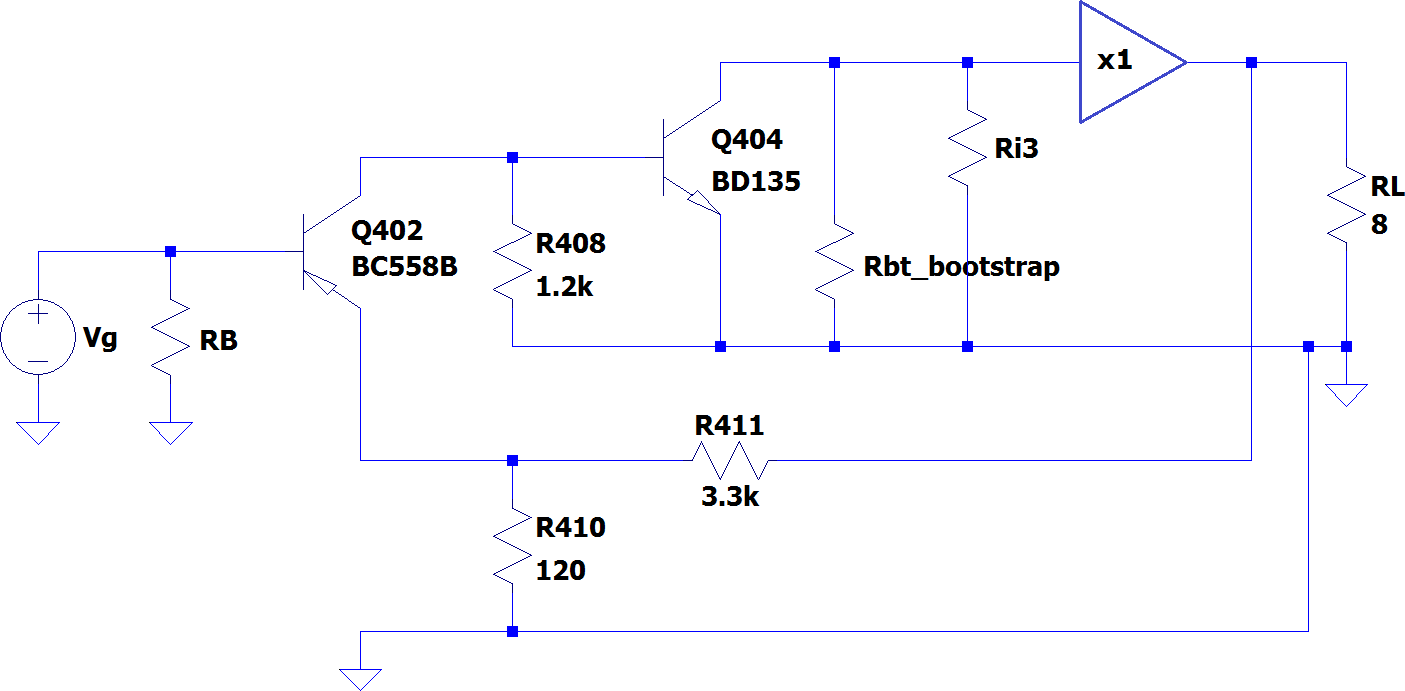
\includegraphics[width=0.75 \textwidth, angle=0]{./img/desarrollo/2_lazo_cerrado.png}
\caption{\label{fig:fig_scheme_signal_circuit}\footnotesize{Circuito de señal esquematizado.}}
\end{center}
\end{figure}

Para poder analizar la ganancia de lazo, es necesaria la ganancia del camino directo, para esto aplicamos \textbf{parámetros híbridos h} al realimentador del circuito, y lo reorganizamos para llevarlo a la forma ideal, lo que se obtiene se muestra en figura~\figref{fig:fig_scheme_signal_circuit_h_parameters}.


\begin{figure}[H] %htb
\begin{center}
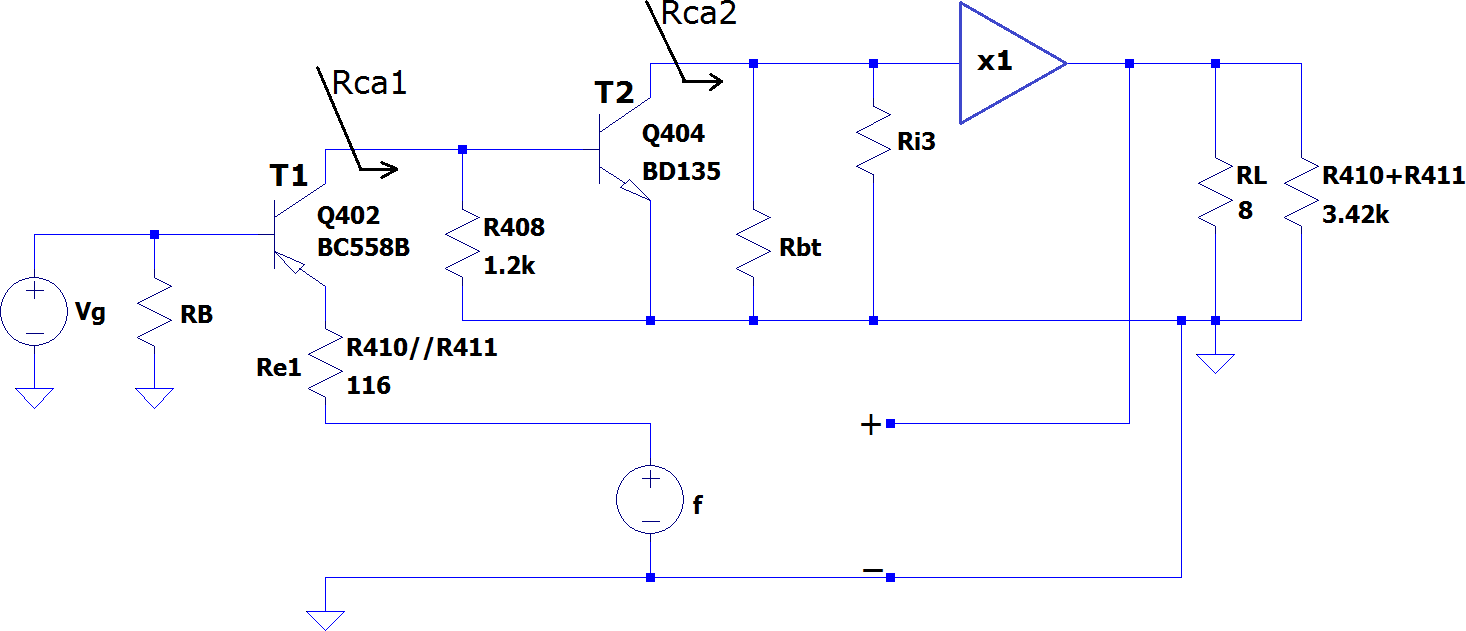
\includegraphics[width=0.75 \textwidth, angle=0]{./img/desarrollo/2-lazoCerradoIdeal.png}
\caption{\label{fig:fig_scheme_signal_circuit_h_parameters}\footnotesize{Circuito de señal esquematizado aplicando parámetros h al realimentador.}}
\end{center}
\end{figure}

\clearpage

\label{calculation_of_f}

\begin{sloppypar}
Donde el parámetro $h_{11} = R_{410} \parallelresistors R_{411} $ queda como resistor de emisor de $Q_{402}$ y $h_{22} = R_{410} + R_{411} $ queda en paralelo con la carga, se desprecia el efecto de $h_{21}$, que es el efecto de la entrada en la salida a través de la realimentación.\\

Se tiene además que $f = h_{12} = \frac{R_{410}}{R_{410} + R_{411}} = \frac{120 \si[per-mode=symbol]{\ohm}}{120 \si[per-mode=symbol]{\ohm} + 3.3 \si[per-mode=symbol]{\kilo\ohm}} \approx 0.035  $
\end{sloppypar}

\subsubsection{Ganancia a lazo abierto del amplificador (\quotemarks{$a$})}
\label{stages_gain}

Para calcular la ganancia del camino directo, ganancia a lazo abierto del amplificador (\textbf{\quotemarks{a}}), se desactiva la realimentación haciendo $f = 0$, el amplificador resultante es la cascada de los dos emisores comunes y la etapa de salida, incluyendo el efecto de carga del realimentador. Todos los cálculos se realizan por inspección, pero teniendo cuidado de usar aproximaciones solo cuando estas sean válidas.\\

La ganancia total será el producto de las ganancias de las tres etapas y no consideramos atenuación en la entrada por calcular suponiendo un generador ideal:\\

\begin{equation}
a = A_{V_{1}} \cdot A_{V_{2}} \cdot A_{V_{3}}
\end{equation}\\





\begin{sloppypar}
Para $A_{V_{1}}$, se cumple que $\beta \gg 1 \; \land \; r_{o} \gg R_{E} \; \land \; gm \cdot r_{o} \gg 1$, podemos usar entonces la expresión aproximada para $A_{V}$: 

$A_{V} \approx -\frac{gm}{1 + gm \cdot R_{E}} \cdot R_{ca}$,  queda entonces:
\end{sloppypar}

\begin{equation}
A_{V_{1}} -\approx \frac{gm_{402}}{1 + gm_{402} \cdot \left( R_{410} \parallelresistors R_{411}\right) } \cdot R_{ca_{1}} = -\frac{gm_{402}}{1 + gm_{402} \cdot \left( R_{410} \parallelresistors R_{411}\right) } \cdot \left( R_{408} \parallelresistors r_{\pi_{404}} \right) \approx -1.8
\end{equation}\\


\begin{sloppypar}
Para $A_{V_{2}}$, tenemos la ganancia de un emisor común: 
\end{sloppypar}


\begin{equation}
A_{V_{2}} = -gm_{404} \cdot R_{ca_{2}} = -gm_{404} \cdot \left(  r{o_{404}} \parallelresistors R_{bt} \parallelresistors R_{i_{3}}  \right)
\end{equation}\\


\begin{sloppypar}
En la figura~\figref{fig:fig_scheme_signal_circuit_h_parameters}, $R_{i_{3}}$ representa la resistencia de entrada de la etapa de salida, y $R_{bt}$ la resistencia que el circuito \mbox{\textbf{bootstrap}} presenta a la segunda etapa, esta última se obtiene en forma aproximada por reflexión de \mbox{\textbf{Miller}} como $R_{bt} = \frac{1}{1 - A_{V_{3}}} \cdot R_{414} $.
La $R_{i_{3}}$ es un tanto mas difícil de calcular, ya que la etapa de salida no funciona en \textbf{clase A}, pero dado que es \textbf{clase AB}, se puede hacer una aproximación suponiendo que se trata de un seguidor por emisor construido alrededor de un \textbf{par Darlington}, en este caso la etapa ni siquiera es completamente simétrica, ya que el papel de transistor \textbf{PNP}, lo cumple un \textbf{par Sziklai}, pero como aproximación para el cálculo manual no es mucho mas lo que se puede hacer, podemos decir que el $\beta$ efectivo del segundo transistor se ve disminuido un poco por la resistencia conectada en su base, teniendo en cuenta esto, aproximamos la resistencia de entrada de la etapa de potencia, como:

\begin{equation*}
R_{i_{3}} = \beta_{405} \cdot \beta_{405_{eff}} \cdot R_{L} \approx \beta_{405} \cdot gm_{407} \cdot \left( r_{\pi_{407}} \parallelresistors R_{419} \right) \cdot R_{L} = 35.56 \si[per-mode=symbol]{\kilo\ohm}
\end{equation*}

Para la ganancia de tensión de la etapa de salida, nuevamente por lo anteriormente dicho, es difícil calcular manualmente un valor, sin embargo por tratarse aproximadamente de un seguidor formado por pares compuestos, asumimos un valor de $A_{V_{3}} = 0.99$, se obtiene valor muy cercano para el \textbf{par Sziklai} realizando todos los cálculos, no tanto para el \textbf{par Darlington}.\\

Las simulaciones nos dirán que tan cercanas a la realidad son estas suposiciones.

\end{sloppypar}


\clearpage


Tenemos entonces:

\begin{equation*}
R_{bt} \approx \frac{1}{1 - A_{V_{3}}} \cdot R_{414} \approx \frac{1}{1 - 0.99} \cdot 2.2 \si[per-mode=symbol]{\kilo\ohm} = 220 \si[per-mode=symbol]{\kilo\ohm}
\end{equation*}


Nos queda entonces:

\label{calculation_of_a}

\begin{equation}
A_{V_{2}} = -gm_{404} \cdot R_{ca_{2}} = -gm_{404} \cdot \left(  r{o_{404}} \parallelresistors R_{bt} \parallelresistors R_{i_{3}}  \right) = -360 \si[per-mode=symbol]{\milli\ampere\per\volt} \cdot \left( 15.9 \si[per-mode=symbol]{\kilo\ohm} \parallelresistors 220 \si[per-mode=symbol]{\kilo\ohm} \parallelresistors 35.56 \si[per-mode=symbol]{\kilo\ohm}  \right) \approx -3770
\end{equation}\\

Con esto, tenemos:

\begin{equation}
a = A_{V_{1}} \cdot A_{V_{2}} \cdot A_{V_{3}} = -1.8 \cdot -3770 \cdot 0.99 \approx 6718
\end{equation}\\


\label{loop_gain}

Finalmente para la ganancia de lazo del amplificador tenemos:

\begin{equation}
\boxed {T = a \cdot f = 6718 \cdot 0.035 \approx 221 }
\end{equation}



\vfill

\clearpage
